\documentclass[12pt, twoside]{article}
%\documentclass[12pt, twoside]{article}
\usepackage[letterpaper, margin=1in, headsep=0.2in]{geometry}
\setlength{\headheight}{0.6in}
%\usepackage[english]{babel}
\usepackage[utf8]{inputenc}
\usepackage{microtype}
\usepackage{amsmath}
\usepackage{amssymb}
%\usepackage{amsfonts}
\usepackage[nomessages]{fp} %\FPeval{\var-name}{2*sin(pi/6)}
\usepackage{siunitx} %units in math. eg 20\milli\meter
\usepackage{yhmath} % for arcs, overparenth command
\usepackage{tikz} %graphics
\usetikzlibrary{quotes, angles, arrows, arrows.meta}
\usepackage{pgfplots}
\usepgfplotslibrary{fillbetween}
\pgfplotsset{compat=1.16}
\usepackage{graphicx} %consider setting \graphicspath{{images/}}
\usepackage{parskip} %no paragraph indent
\usepackage{enumitem}
\usepackage{multicol}
\usepackage{venndiagram}

\usepackage{fancyhdr}
\pagestyle{fancy}
\fancyhf{}
\renewcommand{\headrulewidth}{0pt} % disable the underline of the header
\raggedbottom
\hfuzz=2mm %suppresses overfull box warnings

\usepackage{hyperref}

\fancyhead[LO]{La Scuola d'Italia / Dr.\ Huson / IB Math 12 \\* 14 October 2026}
\fancyhead[RO]{\fbox{\begin{minipage}{6cm}\footnotesize Nickname:\\[0.5cm]\end{minipage}}}
\fancyhead[LE]{\fbox{\begin{minipage}{6cm}\footnotesize Nickname:\\[0.5cm]\end{minipage}}}
\fancyfoot[C]{\thepage}

\pgfplotsset{
  cfgraph/.style={
    grid=both,
    major grid style={black!45},
    minor grid style={black!18},
    axis lines=left,
    enlargelimits=false,
    width=12cm,
    height=7.2cm,
    tick label style={font=\footnotesize},
    label style={font=\footnotesize},
  }
}

\begin{document}
\subsubsection*{1.11 Quiz: Statistics}

\begin{enumerate}[itemsep=0.15cm]

%--- Problem 1: Grouped frequency table; continuous data; modal class; estimated mean and sd; stratified sample [7 marks] ---
%--- Source: Original (freshly authored, AA SL 4.1, 4.2, 4.3); parallel of 1-10PQ_Statistics P1 (no "explain why estimate" part) ---
\item[1.] [Maximum mark: 7]

The table shows the waiting time, $t$ minutes, of $50$ patients at a
clinic.

\begin{center}
\setlength{\tabcolsep}{3.5pt}\renewcommand{\arraystretch}{1.2}
\begin{tabular}{|l|c|c|c|c|c|}
\hline
Time, $t$ & $0 \le t < 10$ & $10 \le t < 20$ & $20 \le t < 30$ & $30 \le t < 40$ & $40 \le t < 50$ \\
\hline
Number of patients & 4 & 12 & 18 & 11 & 5 \\
\hline
\end{tabular}
\end{center}

\begin{enumerate}[itemsep=0.1cm]
  \item State whether the data are discrete or continuous. \hfill [1]
  \item Write down the modal class. \hfill [1]
  \item Find an estimate of the mean waiting time. \hfill [2]
  \item Find an estimate of the standard deviation. \hfill [1]
  \item The $50$ patients are a stratified sample, by age group, of the
  $600$ patients registered at the clinic. There are $192$ registered
  patients over the age of $65$. Find the number of patients over the age
  of $65$ in the sample. \hfill [2]
\end{enumerate}

\begin{tikzpicture}
  \draw (-0.6,0) rectangle (14.6,12.6);
  \foreach \y in {1,2,...,12} \draw[dotted] (0,\y)--(14.1,\y);
\end{tikzpicture}

\newpage

%--- Problem 2: Five-number summary from raw data; IQR; low-outlier test; draw the box plot [9 marks] ---
%--- Source: Original (freshly authored, AA SL 4.2); parallel of 1-10PQ_Statistics P2 (outlier at the low end) ---
\item[2.] [Maximum mark: 9]

Fifteen students recorded the number of push-ups they could do in one
minute.

\begin{center}
$27,\; 31,\; 22,\; 35,\; 28,\; 25,\; 33,\; 8,\; 29,\; 24,\; 36,\; 26,\;
30,\; 28,\; 32$
\end{center}

\begin{enumerate}[itemsep=0.1cm]
  \item Write down the median, the lower quartile $Q_{1}$ and the upper
  quartile $Q_{3}$. \hfill [2]
  \item Find the interquartile range. \hfill [1]
  \item Show that $8$ is an outlier. \hfill [3]
  \item On the scale at the bottom of the box, draw a box-and-whisker
  plot of the data. Mark the outlier with a cross. \hfill [3]
\end{enumerate}

\begin{tikzpicture}
  \draw (-0.6,0) rectangle (14.6,15.0);
  \foreach \y in {5,6,...,14} \draw[dotted] (0,\y)--(14.1,\y);
  \begin{scope}[xshift=-1.15cm, x=0.35cm]
    \foreach \t in {5,10,...,40} \draw[dotted] (\t,1.4)--(\t,4.2);
    \draw (5,1.4)--(41,1.4);
    \foreach \t in {5,6,...,41} \draw (\t,1.32)--(\t,1.48);
    \foreach \t in {5,10,...,40} \draw (\t,1.22)--(\t,1.58);
    \foreach \t in {5,10,...,40} \node[below] at (\t,1.2) {\footnotesize \t};
    \node at (23,0.35) {\footnotesize Number of push-ups};
  \end{scope}
\end{tikzpicture}

\newpage

%--- Problem 3: Read median, IQR, a count and a percentile from a CF curve; frequencies from the curve [9 marks] ---
%--- Source: Original (freshly authored, AA SL 4.2); parallel of 1-10PQ_Statistics P3 ---
\item[3.] [Maximum mark: 9]

The cumulative frequency graph shows the lengths, $L$ cm, of $200$ fish
caught in a river.

\begin{center}
\begin{tikzpicture}
\begin{axis}[cfgraph,
  xlabel={Length, $L$ (cm)},
  ylabel={Cumulative frequency},
  xmin=0, xmax=60, ymin=0, ymax=200,
  xtick={0,10,...,60}, ytick={0,20,...,200},
  minor x tick num=4, minor y tick num=3,
]
% Solution curve: cf(20)=30, Q1=24 (cf 50), cf(28)=75, median=32 (cf 100), Q3=40 (cf 150), cf(44)=170
\addplot[smooth, thick, no markers] coordinates {
  (0,0) (8,4) (16,15) (20,30) (24,50) (28,75) (32,100) (36,125) (40,150)
  (44,170) (48,185) (52,193) (56,198) (60,200)
};
\end{axis}
\end{tikzpicture}
\end{center}

\begin{enumerate}[itemsep=0.02cm]
  \item Write down the median length. \hfill [1]
  \item Find the interquartile range. \hfill [2]
  \item Find the number of fish longer than $44$ cm. \hfill [2]
  \item The shortest $15\%$ of the fish are returned to the river. Find
  the greatest length of a fish that is returned. \hfill [2]
  \item The lengths are grouped in the table below. Find the values of
  $p$ and $q$. \hfill [2]
\end{enumerate}

\begin{center}
\setlength{\tabcolsep}{8pt}\renewcommand{\arraystretch}{1.2}
\begin{tabular}{|l|c|c|c|c|}
\hline
Length, $L$ (cm) & $0 < L \le 20$ & $20 < L \le 28$ & $28 < L \le 44$ & $44 < L \le 60$ \\
\hline
Number of fish & 30 & $p$ & $q$ & 30 \\
\hline
\end{tabular}
\end{center}

\begin{tikzpicture}
  \draw (-0.6,0) rectangle (14.6,7.6);
  \foreach \y in {1,2,...,7} \draw[dotted] (0,\y)--(14.1,\y);
\end{tikzpicture}

\newpage

%--- Problem 4: Pearson's r, characterizing correlation, y-on-x regression line, interpreting the gradient, interpolation [8 marks] ---
%--- Source: Original (freshly authored, AA SL 4.4); parallel of 1-10PQ_Statistics P4 (negative correlation; no extrapolation part) ---
\item[4.] [Maximum mark: 8]

The table shows the age, $x$ years, and the price, $y$ thousand dollars,
of eight used cars of the same model.

\begin{center}
\setlength{\tabcolsep}{7pt}\renewcommand{\arraystretch}{1.2}
\begin{tabular}{|l|c|c|c|c|c|c|c|c|}
\hline
Age, $x$ (years) & 1 & 2 & 3 & 5 & 6 & 8 & 9 & 10 \\
\hline
Price, $y$ (thousand dollars) & 27 & 27 & 22 & 21 & 16 & 15 & 11 & 12 \\
\hline
\end{tabular}
\end{center}

\begin{enumerate}[itemsep=0.1cm]
  \item Find Pearson's product-moment correlation coefficient, $r$.
  \hfill [1]
  \item Characterize the correlation (positive or negative; strong,
  moderate, weak, or none). \hfill [2]
  \item Write down the regression line of $y$ on $x$, in the form
  $y = ax + b$. \hfill [2]
  \item Interpret the meaning of the value of $a$ in this context.
  \hfill [1]
  \item Use your regression line to estimate the price of a car that is
  $7$ years old. \hfill [2]
\end{enumerate}

\begin{tikzpicture}
  \draw (-0.6,0) rectangle (14.6,13.8);
  \foreach \y in {1,2,...,13} \draw[dotted] (0,\y)--(14.1,\y);
\end{tikzpicture}

\end{enumerate}
\end{document}
